%!TEX root = 
% Тип документа
\documentclass[a4paper,12pt]{extarticle}

% Шрифты, кодировки, символьные таблицы, переносы
% \usepackage{cmap}
% \usepackage[T2A]{fontenc}
\usepackage[utf8]{inputenc}
\usepackage[russian]{babel}
% Это пакет -- хитрый пакет, он нужен но не нужен
\usepackage[mode=buildnew]{standalone}

\usepackage
	{
		% Дополнения Американского математического общества (AMS)
		amssymb,
		amsfonts,
		amsmath,
		amsthm,
		% Пакет для физических текстов
		physics,
		% misccorr,
		% 
		% Графики и рисунки
		wrapfig,
		graphicx,
		subcaption,
		float,
		caption,
		color,
		booktabs,
		geometry,
		% 
		% Таблицы, списки
		makecell,
		multirow,
		indentfirst,
		%
		% Интегралы и прочие обозначения
		ulem,
		esint,
		esdiff,
		% 
		% Колонтитулы
		fancyhdr,
	} 
    
\usepackage{mathtools}
\mathtoolsset{showonlyrefs=true} 
\usepackage{pgfplots,pgfplotstable,booktabs,colortbl}
\usepackage{xcolor}
\usepackage{hyperref}
\usepackage{pythontex}
 % Цвета для гиперссылок
\definecolor{linkcolor}{HTML}{000000} % цвет ссылок
\definecolor{urlcolor}{HTML}{799B03} % цвет гиперссылок
 
\hypersetup{pdfstartview=FitH,linkcolor=linkcolor,urlcolor=urlcolor, colorlinks=true}
\hypersetup{pageanchor=false}
% Увеличенный межстрочный интервал, французские пробелы
\linespread{1.3} 
\frenchspacing 

\newcommand{\mean}[1]{\langle#1\rangle}

\begin{pycode}
##
def frexp10(decimal):
	parts = ('%e' % decimal).split('e')
	return float(parts[0]), int(parts[1])
##
\end{pycode}



% Функция для тех, кто использует pythontex. Представляет любое вещественное число в стандартном виде.
\newcommand{\frexp}[1]{
		\pyc{#10=frexp10(#1)} 
			\py{ round(#10[0],2)} 
				\cdot 10^{\py{#10[1]}} }

% const прямым шрифтом
\newcommand\ct[1]{\text{\rmfamily\upshape #1}}
\newcommand*{\const}{\ct{const}}
\usepackage{array}
\usepackage{pstool}

\geometry		
	{
		left			=	2cm,
		right 			=	2cm,
		top 			=	2.5cm,
		bottom 			=	2.5cm,
		bindingoffset	=	0cm
	}

%%%%%%%%%%%%%%%%%%%%%%%%%%%%%%%%%%%%%%%%%%%%%%%%%%%%%%%%%%%%%%%%%%%%%%%%%%%%%%%
	%применим колонтитул к стилю страницы
\pagestyle{fancy} 
	%очистим "шапку" страницы
% \fancyhead{} 
	%слева сверху на четных и справа на нечетных
\fancyhead[R]{}%\labauthors 
	%справа сверху на четных и слева на нечетных
% \fancyhead[L]{Отчёт по лабораторной работе №\labnumber}
\fancyhead[L]{\labtheme} 
	%очистим "подвал" страницы
% \fancyfoot{} 
	% номер страницы в нижнем колинтуле в центре
\fancyfoot[C]{\thepage} 

%%%%%%%%%%%%%%%%%%%%%%%%%%%%%%%%%%%%%%%%%%%%%%%%%%%%%%%%%%%%%%%%%%%%%%%%%%%%%%%

\renewcommand{\contentsname}{Оглавление}
\usepackage{tocloft}
\usepackage{secdot}
\sectiondot{subsection}



\begin{document}

\def\labauthors{Войтович Д.А., Понур К.А.}
\def\labgroup{440}
\def\labnumber{1}
\def\labtheme{Исследование влияния пространственного заряда на прохождение тока в диоде}
\def\department{Кафедра общей физики}
\renewcommand{\vec}{\mathbf}
\renewcommand{\phi}{\varphi}
\renewcommand{\hat}{\widehat}

\begin{titlepage}

\begin{center}

{\small\textsc{Нижегородский государственный университет имени Н.\,И. Лобачевского}}
\vskip 1pt \hrule \vskip 3pt
{\small\textsc{Радиофизический факультет}}



\vfill
{\Large {\department}}

{\Large Отчет по лабораторной работе №\labnumber\vskip 12pt\bfseries \labtheme}
	
\end{center}

\vfill
	
\begin{flushright}
	{Выполнили студенты \labgroup\ группы\\ \labauthors}%\vskip 12pt Принял:\\ Менсов С.\,Н.}
\end{flushright}
	
\vfill
	
\begin{center}
	Нижний Новгород, \the\year
\end{center}

\end{titlepage}



\section{Теоретическая часть}
\subsection{Основные режимы работы диода}
Пусть поперечные размеры анода и катода $L_y,L_z \gg d$ - расстояния между катодом и анодом. Тогда зависимостью всех величин от x, z можно пренебречь и считать, что потенциал, электрическое поле, скорость зависят только от координаты x, отсчитываемой от катода к аноду. Будем полагать $U_k=0, U_a=const > 0$.

\begin{figure}[h!]
    \centering
    \includegraphics[width=0.35\linewidth]{fig/img8062.jpg}
    \caption{Плоский диод}
    \label{fig:1}
\end{figure}

Предположим, эмиссионная способность катода может неограниченно расти при увеличении T, начальная скорость электронов $V_0=0$.

Если температура невелика, то пространственный заряд в диоде и его поле $E_{\rho}$ малы, поэтому и электрическое поле $E_x=E$ для электрона на всем промежутке анод-катод остается ускоряющим. Все электроны с катода доходят до анода - это режим насыщения (режим температурного ограничения эмиссии), поскольку в этом случае ток через диод полностью определяются температурой катода.

Рассмотрим распределение потенциала. Выделим из потока электронов плоский слой толщиной $dx$. Электроны заряжены отрицательно, собственное кулоновское поле слоя $E_{\rho}$ направлено к слою. Поле зарядов на электродах $E_{el}$ - от анода к катоду. В результате слева от слоя эти поля направлены в противоположные стороны и вычитаются, а справа - в одну сторону и складываются. 
\begin{figure}[h!]
    \centering
    \includegraphics[width=0.5\linewidth]{fig/img8063.jpg}
    \caption{Распределение потенциала в плоском диоде при различной температуре катода T: 1-T=0, 2-T=$T_1$, 3-T=$T_3$, 4-T=$T_4$, 5-случай $U_a<0$}
    \label{fig:2}
\end{figure}
\begin{figure}[h!]
    \centering
    \includegraphics[width=0.5\linewidth]{fig/img8064.jpg}
    \caption{Распределение поля и потенциала в диоде}
    \label{fig:3}
\end{figure}

При увеличении температуры кривая начинает провисать, и после достижения некоторого значения распределение поля, потенциала и пространственного заряда перестает меняться. Не будет меняться и ток через диод, а будет определяться только потенциалом анода. Такой режим работы называется режимом ограничения тока пространственным зарядом. 

При $U_a<0$ между катодом и анодом возникает тормозящее поле. Если бы электроны не обладали начальными тепловыми скоростями, то они не смогли бы преодолеть барьер, и ток анода был был равен нулю. Скорости электронов имеют максвелловское распределение, откуда следует, что анодный ток будет экспоненциально убывающей функцией $|U_a|$. Режим работы при $U_a<0$ получил название режима начальных токов.

\subsection{Режим ограничения тока пространственным зарядом}
Изучим зависимость анодного тока $J_a$ от анодного напряжения $U_a$ для плоского диода в стационарном режиме, когда все переходные процессы, возникающие при включении диода, уже завершены. 
\begin{equation}
    J_a=PU_a^{3/2}.
\end{equation}

Это закон "трех-вторых". Величина P - преверанс диода. Независимо от геометрии  диодов качественное поведение этих систем при изменении температуры катода должно быть сходным с плоским диодом, поскольку основное влияние на величину тока оказывает узкая прикатодная область, где скорости электронов малы, а плотность объемного заряда- велика. В этом случае кривизна катода слабо сказывается на распределении потенциала в прикатодной области.

\begin{figure}[h!]
    \centering
    \includegraphics[width=0.5\linewidth]{fig/img8072.jpg}
    \caption{Распределение электрического поля в холодном диоде (1) и в режиме ограничения тока пространственным зарядом (2). Заштрихована область быстрого изменения поля}
    \label{fig:4}
\end{figure}

\subsection{Ток диода в режиме насыщения}

\begin{figure}[h!]
    \centering
    \includegraphics[width=0.5\linewidth]{fig/img80825.jpg}
    \caption{Образование поля дипольного слоя на границе металла. Стрелками указано направление поля}
    \label{fig:5}
\end{figure}

\begin{figure}[h!]
    \centering
    \includegraphics[width=0.5\linewidth]{fig/img8083.jpg}
    \caption{Распределение электрического поля в холодном диоде (1) и в режиме ограничения тока пространственным зарядом (2). Заштрихована область быстрого изменения поля}
    \label{fig:6}
\end{figure}

Все электроны, эмитированные с катода, оказываются в ускоряющем поле и доходят до анода. При малых напряженностях на выходящий из твердого тела электрон последовательно действуют две возвращающие силы: сила дипольного слоя (на малых расстояниях) и сила зеркального изображения (на больших). Если электрон отошел от поверхности на расстояние, много большее межатомного расстояния, то неоднородностью поверхности можно пренебречь и считать, что электрон находится над плоской поверхностью идеального проводника. 
Ток термоэмиссии:
\begin{equation}
J_a=S_a A T^2 e^{-e \phi /kT},
\end{equation}
где А-эмиссионная константа, $\phi$ - эффективная работа выхода. Прологарифмируем:
\begin{equation}
lnJ_a-2lnT=ln(s-a \cdot A)-\frac{e\phi}{kT}.
\end{equation}

Если менять температуру и изменять анодный ток $J_s$, то, откладывая по осям $lnJ_a-2lnT$ и $1/T$, получим прямую Ричардсона по наклону которой определяется $\phi$.

\begin{figure}[H]
    \centering
    \includegraphics[width=0.75\linewidth]{fig/img8084.jpg}
    \caption{Распределение суммарного электрического поля, действующего на выходящий из твердого тела электрон}
    \label{fig:7}
\end{figure}

\begin{figure}[h!]
    \centering
    \includegraphics[width=0.75\linewidth]{fig/img8085.jpg}
    \caption{Профиль потенциального барьера на границе твердого тела в случае слабого (1) и сильного (2) электрических полей на катоде}
    \label{fig:8}
\end{figure}

Однако такая формула для тока анода справедлива при малых величинах напряженности поля на катоде. Выше некоторого значения на величину и профиль потенциального барьера начинает оказывать влияние существующее в прикатодной области электрическое поле электродов - проявляется эффект Шоттки. 

Вольт-амперная характеристика диода:
 \begin{figure}[h!]
    \centering
    \includegraphics[width=0.75\linewidth]{fig/img8092.jpg}
    \caption{Вольт-амперная характеристика диода. 1 - режим начальных токов, 2 - режим ограничения тока пространственным зарядом, 3 - режим температурного ограничения эмиссии}
    \label{fig:9}
\end{figure}


\section{Экспериментальная часть}
\subsection{Экспериментальная установка}
Схема установки:
\begin{figure}[h!]
	\centering
	\includegraphics[width=0.5\linewidth]{fig/img9.jpg}
	\caption{Схема экспериментальной установки}
	\label{fig:10}
\end{figure}

Исследуемый трёханодный диод с прямонакальным катодом помещён в защитный корпус (2). Питание накала диода осуществляется источником постоянного тока (3), анодные цепи запитываются от источника постоянного напряжения (4). Для изменения анодного тока диода используется миллиамперметр (1), анодное напряжение индицируется вольтметром, встроенным в источник питания (4), ток и напряжение накала катодной цепи измеряются внутренним прибором источника (3). Для сборки экспериментальных схем используются соединительные провода (6). Блок симметрирующих резисторов (5) позволяет эмулировать подключение минуса анодного питания к середине катода диода.

\begin{figure}[h!]
	\centering
	\includegraphics[width=0.5\linewidth]{fig/img10.jpg}
	\caption{Исследуемый диод}
	\label{fig:11}
\end{figure}

\subsection{Задание 1}
\textit{Установите ток накала 1.42 А, измерьте напряжение накала. Снимите ВАХ
диода в диапазоне напряжений 0...120 В.}

\begin{figure}[h!]
	\centering
	\includegraphics[width=0.4\linewidth]{fig/z1.jpg}
	\caption{К заданию 1}
	\label{fig:12}
\end{figure}



\begin{figure}[H]
	\centering
    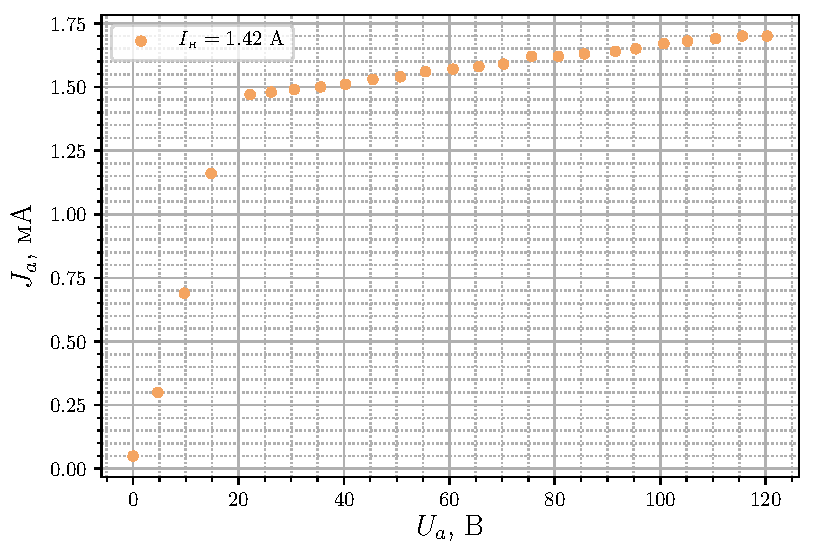
\includegraphics[scale=1]{scripts/fig1}
	\caption{Вольт-амперная характеристика диода при токе накала 1.42 А}
	\label{fig:13}
\end{figure}
\newpage
\subsection{Задание 2}
\textit{Установите ток накала 1.46 А, измерьте напряжение накала. Снимите ВАХ
диода в диапазоне напряжений 0...120 В.}

\begin{figure}[H]
	\centering
	\includegraphics[width=0.4\linewidth]{fig/z2.jpg}
	\caption{К заданию 2}
	\label{fig:14}
\end{figure}


\begin{figure}[H]
	\centering
    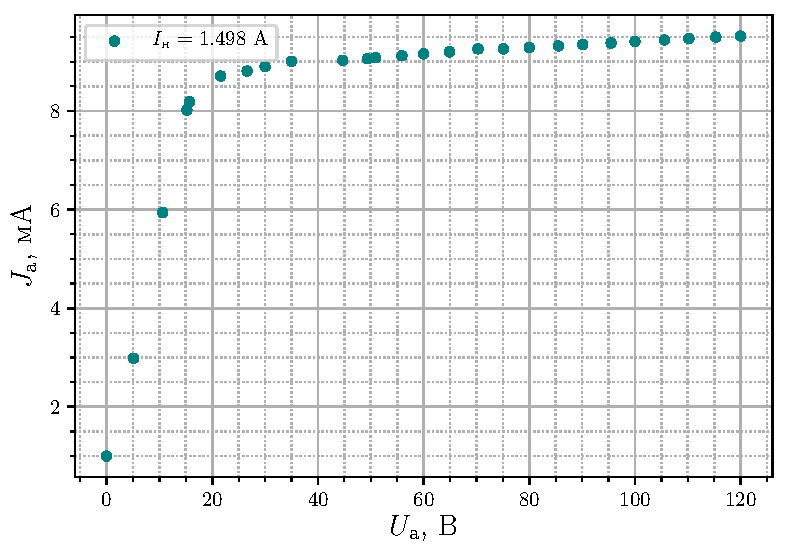
\includegraphics[scale=1]{scripts/fig2}
	\caption{Вольт-амперная характеристика диода при токе накала 1.46 А}
	\label{fig:15}
\end{figure}

\subsection{Задание 3}

\begin{figure}[h!]
	\centering
	\includegraphics[width=0.4\linewidth]{fig/z3.jpg}
	\caption{К заданию 3}
	\label{fig:16}
\end{figure}

\textit{Установите ток накала 1.500 А измерьте напряжение накала. Снимите ВАХ
диода в диапазоне напряжений 0...120 В.}

\begin{figure}[H]
	\centering
    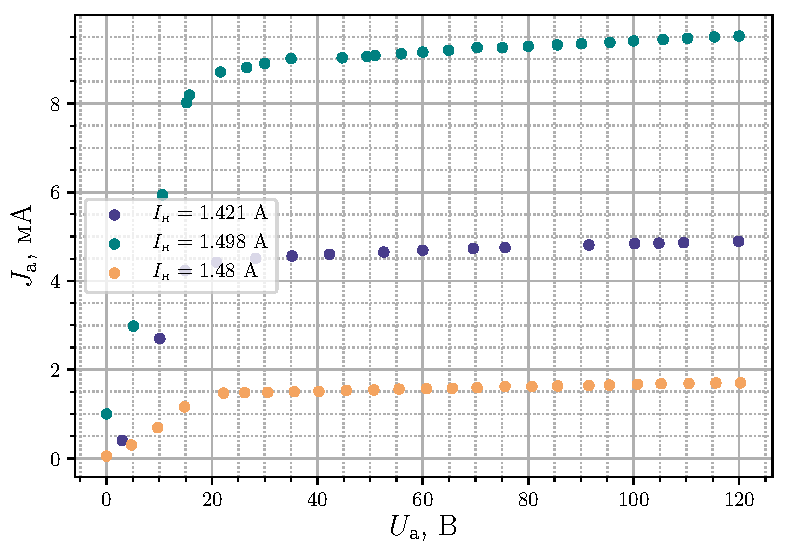
\includegraphics[scale=1]{scripts/fig3}
	\caption{Вольт-амперная характеристика диода при токе различных токах
    накала}
	\label{fig:17}
\end{figure}

\subsection{Задание 4}
Схема та же. Снимите зависимость анодного тока от тока накала при постоянном анодном напряжении (схема рис. 16). Измерения проделать для анодного напряжения 15 В, 60 В, и 100 В.

\begin{figure}[H]
	\centering
    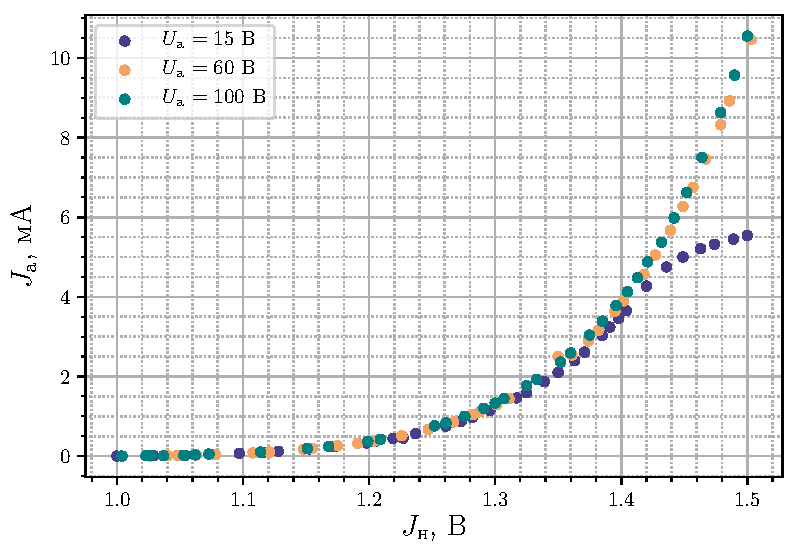
\includegraphics[width=0.85\linewidth]{scripts/fig4}
	\caption{}
	\label{fig:18}
\end{figure}

\subsection{Задание 5}
\textit{По полученным данным постройте прямую Ричардсона (температуру
    определить по таблице Ленгмюра). По прямой Ричардсона вычислите работу
выхода катода.}


С помощью таблицы Ленгмюра [Приложение \ref{sub:tablitsa_lengmiura}] была построена
зависимость температуры от тока накала для вольфрамовой нити длиной $l=$ см и
диаметром  $d = $ см (см. рис. \ref{fig:temperature}). Для упрощения вычислений 
, из таблица Ленгмюра была аппроксиммирована линейной функцией $T(J_{\text{н}})
= \alpha J_{\text{н}} + \beta$ с коэффициентами:
\begin{equation}
    \label{eq:approx_lengmur}
    \alpha = 0.987 \quad \beta = 980
\end{equation}

Тогда формулу для построения прямой Ричардсона можно привести к виду
\begin{equation}
    \label{eq:richardson}
    \ln J_s - 2 \ln(\alpha J_s + \beta )= \ln(S_a A) - \frac{e \phi}{k T}
\end{equation}
С помощью этой зависимости
была построена прямая Ричардсона (см. рис \ref{fig:richardson}). Аппроксимируя
эту прямую линейной функцией, находим значение тангенса угла наклона этой
прямой
\begin{equation}
    - \frac{e \phi}{k} = -120595.5,
\end{equation}
где $e= 1.16\cdot 10^{-19}$ Кл, $k = 1.38\cdot 10^{-23} \text{ Дж} \cdot
\text{К}.$
Отсюда не сложно получить значение эффективной работы выхода $\phi$
 \begin{equation}
     \phi = 9.847 \text{ В}
\end{equation}

\begin{figure}[H]
	\centering
    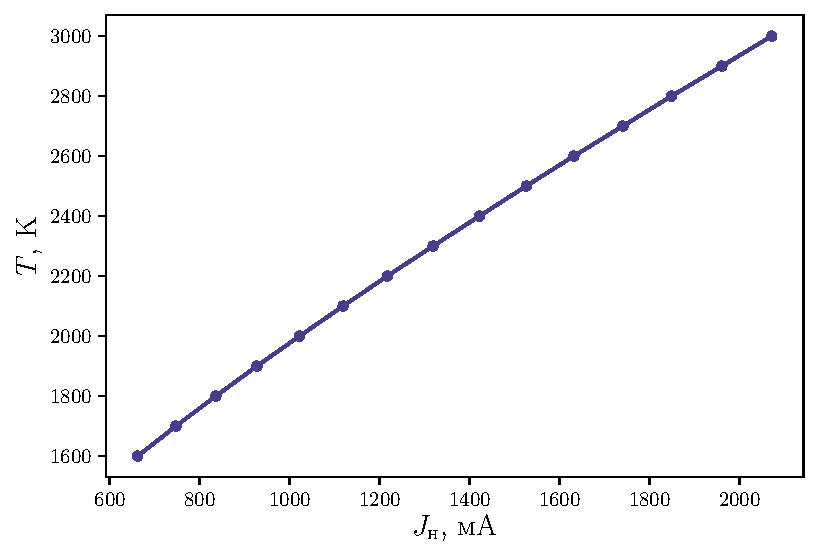
\includegraphics[width=0.75\linewidth]{scripts/lengmur}
	\caption{Зависимость температуры $T$ от тока накала $J_{\text{н}}$}
	\label{fig:temperature}
\end{figure}

\begin{figure}[H]
	\centering
	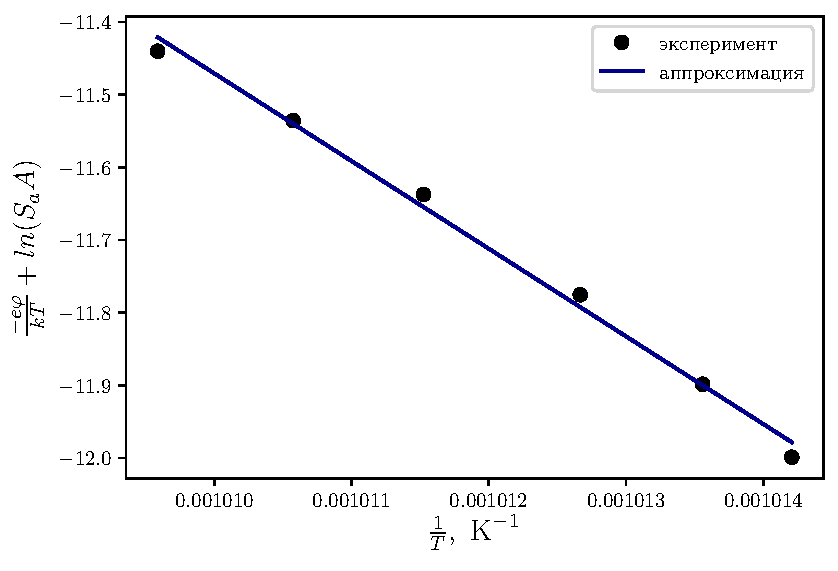
\includegraphics[width=0.75\linewidth]{scripts/richardson}
	\caption{Линейный участок прямой Ричардсона}
	\label{fig:richardson}
\end{figure}

\subsection{Задание 6}
 Постройте теоретические ВАХ для задания 1 по закону “3/2” для эквипотенциального катода и задания 3, используя таблицу значений F(Ua/Uf):
 \begin{figure}[H]
	\centering
	\includegraphics[width=0.65\linewidth]{fig/z71.jpg}
	\caption{}
	\label{fig:21}
\end{figure}

 \begin{figure}[H]
	\centering
	\includegraphics[width=0.65\linewidth]{fig/z72.jpg}
	\caption{}
	\label{fig:22}
\end{figure}
\subsection{Задание 7}
 Для задания 1 вычислите по точкам на экспериментальной кривой удельный заряд электрона. На каком участке ВАХ надо выбирать точки для расчета?

С учетом, что 
\begin{equation}
J_a=\frac49 \varepsilon_0 \sqrt{2 \eta} \frac{S_a}{r_a^2 \beta^2} U^{3/2}, 
\end{equation}
$\beta^2=(1-\frac{r_k}{r_a})^2$, $r_a$= 4 мм, $r_k$= 0.05 мм, $S_a$ - площадь анода, удельный заряд электрона равен $\eta=4.1 \cdot 10^{11}$ кл/кг.


\appendix

\section{Таблица Ленгмюра}%
\label{sub:tablitsa_lengmiura}
При практических расчетах температуры $T$ вольфрамового катода по току накала
$J_{\text{н}}$  удобно пользоваться таблицей, составленной Ленгмюром.

\textbf{
    Следует обратить внимание, что в таблице дана зависимость  $T$ от
    $J'_{\text{н}}$  ($\frac{\text{А}}{\text{см}^3}$) -- приведенного тока
    накала для проволочного вольфрамового катода, длина которого 1 см и диаметр
    1 см. 
} 

Для того чтобы от табличных данных перейти к катоду длина которого $l$ и
диаметр $d$, надо воспользоваться соотношением
\begin{equation}
    \label{eq:lengmur}
    J_{\text{н}} = J'_{\text{н}} d^{3 / 2}
\end{equation}

Выражение \eqref{eq:lengmur} выводится из условия, что мощность рассеиваемая с
1 $\text{см}^2$ при одинаковых рабочих температурах остается постоянной
 \begin{equation}
     \frac{W}{\pi d l} = \frac{J_{\text{н}}^2 R}{\pi d l} = \frac{J^2_{\text{н}}
     \rho \frac{4l}{\pi d^2}}{\pi d l} = \frac{J^2_{\text{н}} 4 \rho}{\pi^2
 d^3} = \frac{(J'_{\text{н}})^2 4 \rho}{\pi^2}
\end{equation}

\begin{table}[h]
    \centering
    \caption{Таблица Ленгмюра}
    \label{tab:lengmur}
    \footnotesize
    \begin{tabular}{||c||c|c|c|c|c|c|c|c|c|c|c|c|c|c|c|}
        \hline
        $J'_{\text{н}}$ & 662.2 & 747.3 & 836   & 927.4 & 1022  & 1119  & 1217  & 1319  & 1422  &
        1526  & 1632  & 1741  & 1849  & 1961  & 2072   \\

        $T$ & 1600 & 1700 & 1800 & 1900 & 2000 & 2100 & 2200 & 2300 & 2400 & 2500 &
        2600 & 2700 & 2800 & 2900 & 3000 \\
        \hline
    \end{tabular}
\end{table}

\end{document}

